\documentclass{beamer}

\usepackage[utf8]{inputenc}
\usepackage{cancel}
\usepackage{amssymb, textcomp,gensymb, lmodern}
% \usetheme{PalotAlto}
% \usecolortheme[named=BurntOrange]

\newcommand{\bi}{\begin{itemize}}
\newcommand{\ei}{\end{itemize}}
\newcommand{\be}{\begin{enumerate}}
\newcommand{\ee}{\end{enumerate}}
\newcommand{\nr}{\cancel{R}}

\usetheme{Berkeley}

\beamertemplatenavigationsymbolsempty

\begin{document}
\title[Two Sample Discrimination]{How do you tell when two samples come from different distributions? }
\author{Chandi Bhandari, Rahul Kumar, Brian Robinson, and Simon Stolarczyk}


\titlepage

\begin{frame}
{Motivating Scenario}

\begin{center}

\includegraphics[scale=.3]{macaque.jpg}
\end{center}

\end{frame}


\begin{frame}
{Motivating Scenario}

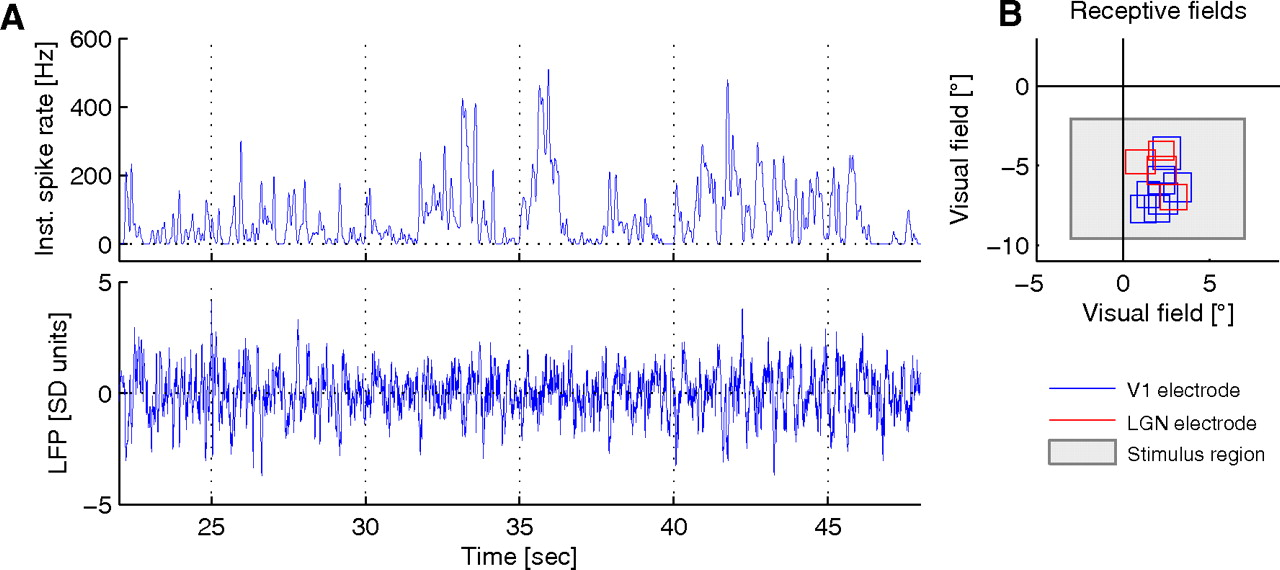
\includegraphics[scale=.32]{lfpspike.jpg}
\end{frame}

%\begin{frame}{Motivating Scenario}
%
%\begin{block}{
%From Gretton et. al.}
%In bioinformatics,  it is of interest to co
%mpare microarray
%data from identical tissue types as measured by different laboratories, to
%detect whether the data
%may be analysed jointly, or whether differences in experimental procedure have caused systematic
%differences in the data distributions.
%\end{block}
%
%\end{frame}


\begin{frame}{Basic Question}

Given two distributions $p$ and $q$, how do we test whether they are different on the basis of samples drawn from each of them?

\begin{center}
$X = (X^1, ... , X^m)$ drawn from $p$

\vspace{.2 cm}

$Y = (Y^1, ..., Y^n)$ drawn from $q$
\end{center}


\end{frame}

\begin{frame}
{Example}

$X = (1.4110420, -0.6491983, -0.2034312,  ...,  0.5670504)$

\vspace{.2 cm}
$Y = ( 2.10555009,  1.59182751,  0.85874229, ...,  0.38632577)$

\pause 

\vspace{1cm}
\begin{center}
$H_0: p = q$

\end{center}
\end{frame}


\begin{frame}{Basic Plotting}

Useful for lower dimensional data, but how do we visualize the difference when $p = N_d(\mu, I)$ when $d >> 3$?

\end{frame}


\begin{frame}{Permutation Testing}

\bi 
\item Develop a statistic given the samples.

\item Permute the samples and run the statistic again.

\item See where the original statistic falls on a plot of the statistic for different permutations. 
\ei 

\end{frame}


\begin{frame}{Kolmogorov-Smirnov Test}

\end{frame}


\section{Gretton et. al. RKHS method}
\begin{frame}{Motivating Fact}
 Expectations over all continuous functions can distinguish probability distributions:
 
 $$p = q \text{ iff. }  E_p[f(x)] = E_q[f(y)] \;\; \forall f \in C(X)$$
\end{frame}

\begin{frame}
{Mean Maximum Discrepancy}

For a set of functions $\mathcal{F}$ define

$$\text{MMD}[\mathcal{F}, p , q] = \sup_{f \in F} ( E_p[f(x)] - E_q[f(y)] )$$
\end{frame}

\begin{frame}
{MMD Estimator}

$$MMD_b [\mathcal{F}, p , q] = \sup_{f \in F} ( \frac 1m \sum_{i = 1}^m f(x_i) - \frac 1n \sum_{i = 1}^n f(y_i) )$$
\end{frame}

\begin{frame}
{How to choose $\mathcal{F}$}

We need something computationally feasible. We want our space $\mathcal{F}$ to be a Hilbert Space with the nice property that taking the expectation of any function is the same as the inner product with some special function 
$$E_xf = \langle f, \mu_p\rangle_\mathcal{H}$$

and we want $$k(x, y) = \langle \phi(x) , \phi(y) \rangle_\mathcal{H}$$

\end{frame}

\begin{frame}{Estimator}

\begin{align*}
{MMD}^2_u[\mathcal{F}, X, Y] &= \frac{1}{m(m-1)}\sum_{i=1}^m\sum_{j \neq i}^m k(x_i, x_j)\\
 &+ \frac{1}{n(n-1)}\sum_{i=1}^n \sum_{j \neq i}^n k(y_i, y_j) \\
 &- \frac{2}{mn}\sum_{i = 1}^m \sum_{j = 1}^n k(x_i, y_j)
\end{align*}  

\end{frame}

\begin{frame}
{Linear Estimator}

$$ {MMD}^2_l[\mathcal{F}, X, Y] = \frac 2m \sum_{i = 1}^{m/2} h((x_{2i -1}, y_{2i - 1}), (x_{2i}, y_{2i}))$$

where $z \sim (x,y), h_(z_i, z_j) := k(x_i, x_j) + k(y_i, y_j) - k(x_i, y_j) - k(x_j, y_i)$
\end{frame}
\begin{frame}{Applying the tests to artificially generated data}
 
\end{frame}

\begin{frame}{Apply the test to experimental data}
 
 \bi
 \item Medical data
 
 \item The distributions for connections on a graph.
 
 \item other from Dr. Fu
 \ei 
\end{frame}





\end{document}
